
\begin{dsaCharacterSheet}
\portraitwp{}

\renewcommand{\arraystretch}{1}
 \setlength{\tabcolsep}{1pt}

\vspace*{4pt}
\begin{dsaSheetBox}[\textwidth]

    \vspace*{-3pt}
    \begin{tabular}{llllllll}
        AT-Basiswert: & \hspace{5pt} \smallnum{\FroEigAktuell{15}} \hspace{10pt} &
        PA-Basiswert: & \hspace{5pt} \smallnum{\FroEigAktuell{16}} \hspace{10pt} &
        FK-Basiswert: & \hspace{5pt} \smallnum{\FroEigAktuell{17}} \hspace{10pt} &
        Initiative-Basiswert: & \smallnum{\FroEigAktuell{14}}
    \end{tabular}
\end{dsaSheetBox}

\vspace{-16pt}
\begin{center}
    \huge \shadowtext{Waffen \& Kampfwerte}%
\end{center}%
\vspace{-8pt}

\newcommand{\Nahkampfwaffen}[2]{%
    \begin{dsaSheetBox}[\textwidth]
        \tiny
        \begin{tabu}{p{4.8cm}|p{2.4cm}|p{1cm}|p{1.4cm}|p{1.6cm}|p{1cm}|p{1.4cm}|p{0.8cm}|p{0.8cm}|p{1.4cm}|p{0.5cm}|p{0.5cm}}
        \dsaTHeading[0]{Nahkampfwaffe} &
        \dsaTHeading{Typ/eBE} &
        \dsaTHeading{DK} &
        \dsaTHeading{TP} &
        \dsaTHeading{TP/KK} &
        \dsaTHeading{INI} &
        \dsaTHeading{WM} &
        \dsaTHeading{AT} &
        \dsaTHeading{PA} &
        \dsaTHeading{TP} &
        \multicolumn{2}{c}{\dsaTHeading[0]{BF}}
        \forloop{ct}{0}{\value{ct} < #1}{%
            \ifcase\value{ct}%
                \\ \Xhline{2\arrayrulewidth}
            \else
                \\ \hline
            \fi
            \mediumtext{\KamNahName{\thect}}{4.8cm} &
            \mediumtext[centered]{\KamNahTypeBE{\thect}}{2.4cm} &
            \mediumtext[centered]{\KamNahDistanzklasse{\thect}}{1cm} &
            \mediumtext[centered]{\KamNahTrefferpunkteBasis{\thect}}{1.4cm} &
            \mediumtext[centered]{\KamNahTPKK{\thect}}{1.6cm} &
            \mediumtext[centered]{\KamNahINIModifikator{\thect}}{1cm} &
            \mediumtext[centered]{\KamNahWaffenmodifikator{\thect}}{1.4cm} &
            \mediumtext[centered]{\KamNahAttacke{\thect}}{0.8cm} &
            \mediumtext[centered]{\KamNahParade{\thect}}{0.8cm} &
            \mediumtext[centered]{\KamNahTrefferpunkte{\thect}}{1.4cm} &
            \mediumtext[centered]{\KamNahBruchfaktora{\thect}}{0.5cm} &
            \mediumtext[centered]{\KamNahBruchfaktorb{\thect}}{0.5cm}
        } \\ \Xhline{3\arrayrulewidth}
        \end{tabu}

        \vspace{2pt}
        \ifthenelse{\equal{#2}{0}}{}{
            \begin{tabular}{p{4cm}p{\textwidth-\fboxsep-\tabcolsep-4cm}} \dsaTHeading[0]{Sonderfertigkeiten} & \mediumtext{\KamSonNahkampf{0}}{\textwidth-\fboxsep-\tabcolsep-4cm}
                \forloop{ct}{1}{\value{ct} < #2}{%
                    \\ \hline
                    \multicolumn{2}{l}{\mediumtext{\KamSonNahkampf{\thect}}{\textwidth-\fboxsep}}%
                }%
            \end{tabular}
        }
    \end{dsaSheetBox}
}

\newcommand{\Fernkampfwaffen}[2]{%
    \begin{dsaSheetBox}[\textwidth]
        \tiny
        \begin{tabu}{p{4.8cm}|p{2.4cm}|p{1.4cm}|p{3.2cm}|p{3.2cm}|p{0.8cm}|p{0.5cm}|p{0.5cm}|p{0.5cm}|p{0.5cm}}
            \dsaTHeading[0]{Fernkampfwaffe} &
            \dsaTHeading{Typ/eBE} &
            \dsaTHeading{TP} &
            \dsaTHeading{Entfernungen} &
            \dsaTHeading{TP/Entfernung} &
            \dsaTHeading{FK} &
            \multicolumn{4}{c}{\dsaTHeading[0]{Geschosse}}
            \forloop{ct}{0}{\value{ct} < #1}{%
                \ifcase\value{ct}%
                    \\ \Xhline{2\arrayrulewidth}
                \else
                    \\ \hline
                \fi
                \mediumtext{\KamFerName{\thect}}{4.8cm} &
                \mediumtext[centered]{\KamFerTypeBE{\thect}}{2.4cm} &
                \mediumtext[centered]{\KamFerTrefferpunkte{\thect}}{1.4cm} &
                \mediumtext[centered]{\KamFerEntfernungen{\thect}}{3.2cm} &
                \mediumtext[centered]{\KamFerTPEntfernung{\thect}}{3.2cm} &
                \mediumtext[centered]{\KamFerFernkampfwert{\thect}}{0.8cm} &
                \mediumtext[centered]{\KamFerGeschossea{\thect}}{0.5cm} &
                \mediumtext[centered]{\KamFerGeschosseb{\thect}}{0.5cm} &
                \mediumtext[centered]{\KamFerGeschossec{\thect}}{0.5cm} &
                \mediumtext[centered]{\KamFerGeschossed{\thect}}{0.5cm}
            } \\ \Xhline{3\arrayrulewidth}
        \end{tabu}

        \vspace{2pt}
        \ifthenelse{\equal{#1}{0}}{}{
            \begin{tabular}{p{4cm}p{\textwidth-\fboxsep-\tabcolsep-4cm}} \dsaTHeading[0]{Sonderfertigkeiten} & \mediumtext{\KamSonFernkampf{0}}{\textwidth-\fboxsep-\tabcolsep-4cm}
                \forloop{ct}{1}{\value{ct} < #2}{%
                    \\ \hline
                    \multicolumn{2}{l}{\mediumtext{\KamSonFernkampf{\thect}}{\textwidth-\fboxsep}}%
                }%
            \end{tabular}
        }
    \end{dsaSheetBox}
}

\newcommand{\Waffenlos}[1]{%
    \begin{dsaSheetBox}[\textwidth]

        \tiny
        \begin{tabu}{p{4.8cm}|p{1.4cm}|p{1cm}|p{1cm}|p{1cm}|p{2.5cm}}
            \dsaTHeading[0]{Waffenloser Kampf} &
            \dsaTHeading{TP/KK} &
            \dsaTHeading{INI} &
            \dsaTHeading{AT} &
            \dsaTHeading{PA} &
            \dsaTHeading{TP(A)} \\ \Xhline{2\arrayrulewidth}
            \forloop{ct}{0}{\value{ct} < 2}{%
                \ifcase\value{ct}\normalfont\small Raufen\or\\\hline\normalfont\small Ringen\fi%
                & \normalfont\small\centering 10/3 &
                \normalfont\small\centering +0 & \mediumtext[centered]{\KamWafAttacke{\thect}}{1cm} &
                \mediumtext[centered]{\KamWafParade{\thect}}{1cm} &
                \mediumtext[centered]{\KamWafTPA{\thect}}{2.5cm}
            } \\ \Xhline{3\arrayrulewidth}
        \end{tabu}

        \vspace{2pt}
        \ifthenelse{\equal{#1}{0}}{}{
            \begin{tabular}{p{4cm}p{\textwidth-\fboxsep-\tabcolsep-4cm}} \dsaTHeading[0]{Sonderfertigkeiten} & \mediumtext{\KamSonWaffenloserKampf{0}}{\textwidth-\fboxsep-\tabcolsep-4cm}
                \forloop{ct}{1}{\value{ct} < #1}{%
                    \\ \hline
                    \multicolumn{2}{l}{\mediumtext{\KamSonWaffenloserKampf{\thect}}{\textwidth-\fboxsep}}%
                }%
            \end{tabular}
        }
    \end{dsaSheetBox}
}

\newcommand{\SchildParierwaffen}[1]{%
    \vspace{-28pt}
    \begin{center}
        \LARGE \shadowtext{Schild / Parierwaffe}%
    \end{center}%
    \vspace{-4pt}

    \begin{dsaSheetBox}
        \tiny
        \begin{tabu}{p{4.8cm}|p{2.6cm}|p{1cm}|p{1.4cm}|p{0.8cm}|p{0.5cm}|p{0.5cm}}
            \dsaTHeading[0]{Name} &
            \dsaTHeading{Typ} &
            \dsaTHeading{INI} &
            \dsaTHeading{WM} &
            \dsaTHeading{PA} &
            \multicolumn{2}{c}{\dsaTHeading[0]{BF}}
            \forloop{ct}{0}{\value{ct} < #1}{%
                \ifcase\value{ct}%
                    \\ \Xhline{2\arrayrulewidth}
                \else
                    \\ \hline
                \fi
                \mediumtext{\KamSchName{\thect}}{4.8cm} &
                \mediumtext[centered]{\KamSchTyp{\thect}}{2.6cm} &
                \mediumtext[centered]{\KamSchINIModifikator{\thect}}{1cm} &
                \mediumtext[centered]{\KamSchWaffenmodifikator{\thect}}{1.4cm} &
                \mediumtext[centered]{\KamSchParade{\thect}}{0.8cm} &
                \mediumtext[centered]{\KamSchBruchfaktora{\thect}}{0.5cm} &
                \mediumtext[centered]{\KamSchBruchfaktorb{\thect}}{0.5cm}
            } \\ \Xhline{3\arrayrulewidth}%
        \end{tabu}

        \vspace{2pt}
        \footnotesize\normalfont\bfseries\centering
        \checkBox[\ui{bgcolor={1 1 1}}\symbolchoice{cross}]{\KamSchLinkhand}{0.13cm}{0.09cm}{on} Linkhand (PA+1),\hspace{5pt}
        \checkBox[\ui{bgcolor={1 1 1}}\symbolchoice{cross}]{\KamSchSchildkampfI}{0.13cm}{0.09cm}{on} Schildkampf I (PA+2)/
        \checkBox[\ui{bgcolor={1 1 1}}\symbolchoice{cross}]{\KamSchSchildkampfII}{0.13cm}{0.09cm}{on} II (PA+2),\hspace{5pt}
        \checkBox[\ui{bgcolor={1 1 1}}\symbolchoice{cross}]{\KamSchParierwaffenI}{0.13cm}{0.09cm}{on} Parierwaffen I/
        \checkBox[\ui{bgcolor={1 1 1}}\symbolchoice{cross}]{\KamSchParierwaffenII}{0.13cm}{0.09cm}{on} II
    \end{dsaSheetBox}
}

\newcommand{\Ruestung}[1]{%
    \begin{center}
        \LARGE \shadowtext{Rüstung}%
    \end{center}%
    \vspace{-4pt}

    \begin{dsaSheetBox}
        \tiny
        \begin{tabu}{p{3.8cm}|p{0.8cm}|p{0.8cm}}
            \dsaTHeading[0]{Rüstungsstück} &
            \dsaTHeading{RS} &
            \dsaTHeading{BE}
            \forloop{ct}{0}{\value{ct} < #1}{%
                \ifcase\value{ct}%
                    \\ \Xhline{2\arrayrulewidth}
                \else
                    \\ \hline
                \fi
                \mediumtext{\KamRusName{\thect}}{4cm} &
                \mediumtext[centered]{\KamRusRustungsschutz{\thect}}{0.8cm} &
                \mediumtext[centered]{\KamRusBehinderung{\thect}}{0.8cm}
            } \\ \Xhline{2\arrayrulewidth}
            \normalfont\bfseries\scriptsize Summe & \mediumtext[centered]{\KamRusSummeRS}{0.8cm} & \mediumtext[centered]{\KamRusSummeBE}{0.8cm} \\ \Xhline{2\arrayrulewidth}
            \multicolumn{2}{l|}{
                \normalfont\scriptsize\bfseries Rüstungsgewöhnung
                \checkBox[\ui{bgcolor={1 1 1}}\symbolchoice{cross}]{\KamRusRustungsgewohnungI}{0.13cm}{0.09cm}{on} I \hspace{1pt}
                \checkBox[\ui{bgcolor={1 1 1}}\symbolchoice{cross}]{\KamRusRustungsgewohnungII}{0.13cm}{0.09cm}{on} II \hspace{1pt}
                \checkBox[\ui{bgcolor={1 1 1}}\symbolchoice{cross}]{\KamRusRustungsgewohnungIII}{0.13cm}{0.09cm}{on} III
            } & \mediumtext[centered]{\KamRusResultierendeBehinderung}{0.8cm}
        \end{tabu}
    \end{dsaSheetBox}
}

\newcommand{\Ausweichen}{%
    \begin{center}
        \LARGE \shadowtext{Ausweichen}%
    \end{center}%
    \vspace{-4pt}

    \begin{dsaSheetBox}
        \setlength{\tabcolsep}{0pt}
        \tiny\normalfont\bfseries
        \begin{tabular}{p{1cm}p{0.3cm}p{0.7cm}p{0.3cm}p{2.5cm}p{0.3cm}p{1cm}}
            \multicolumn{2}{l}{\scriptsize PA-Basis} & \scriptsize\centering BE & & \scriptsize\centering SF Ausweichen & & \scriptsize Summe \\
            \textField[\ui{align={centered},textsize={14}}\Ff{\FfReadOnly}]{PA-akt}{1cm}{18pt} &
            \normalsize $-$ &
            \textField[\ui{align={centered},textsize={14}}\Ff{\FfReadOnly}]{BE}{0.7cm}{18pt} &
            \normalsize $+$ &
            \begin{minipage}{2.5cm}
                \centering
                \checkBox[\ui{bgcolor={1 1 1}}\symbolchoice{cross}]{\KamAusAusweichenI}{0.13cm}{0.09cm}{on} I \hspace{1pt}
                \checkBox[\ui{bgcolor={1 1 1}}\symbolchoice{cross}]{\KamAusAusweichenII}{0.13cm}{0.09cm}{on} II \hspace{1pt}
                \checkBox[\ui{bgcolor={1 1 1}}\symbolchoice{cross}]{\KamAusAusweichenIII}{0.13cm}{0.09cm}{on} III \hspace{1pt} \\
                jeweils +3 \\
                Flink (+1) / Behäbig (-1)?
            \end{minipage}
             & \normalsize $=$ &
            \textField[\ui{align={centered},textsize={14}}]{\KamAusAusweichenwert}{0.9cm}{18pt} \\ \Xcline{1-1}{3\arrayrulewidth} \Xcline{3-3}{3\arrayrulewidth} \Xcline{7-7}{3\arrayrulewidth}
             & & & \multicolumn{3}{c}{Akrobatik (+$\lfloor(\mathrm{TaW}-9) / 3 \rfloor $)?} &
        \end{tabular}
    \end{dsaSheetBox}
}

\newcommand{\Wunden}{%
    \begin{center}
        \LARGE \shadowtext{Wunden}%
    \end{center}%
    \vspace{-3pt}

    \begin{dsaSheetBox}
        \centering
        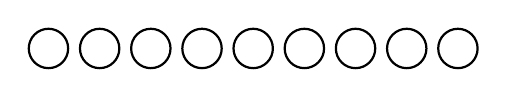
\begin{tikzpicture}
            \filldraw[fill=white, draw=black, thick] (1,1) circle (0.25cm);
            \filldraw[fill=white, draw=black, thick] (1.65,1) circle (0.25cm);
            \filldraw[fill=white, draw=black, thick] (2.3,1) circle (0.25cm);
            \filldraw[fill=white, draw=black, thick] (2.95,1) circle (0.25cm);
            \filldraw[fill=white, draw=black, thick] (3.6,1) circle (0.25cm);
            \filldraw[fill=white, draw=black, thick] (4.25,1) circle (0.25cm);
            \filldraw[fill=white, draw=black, thick] (4.9,1) circle (0.25cm);
            \filldraw[fill=white, draw=black, thick] (5.55,1) circle (0.25cm);
            \filldraw[fill=white, draw=black, thick] (6.2,1) circle (0.25cm);
        \end{tikzpicture} \\
        \scriptsize\normalfont\bfseries je Wunde AT, PA, FK, GE, INI - 2, GS - 1
    \end{dsaSheetBox}
}

\newcommand{\dsaTSHeading}[1]{\centering\normalfont\bfseries\scriptsize #1}

\newcommand{\LebensenergieAusdauerEtc}[2]{
    \begin{center}%
        \LARGE \shadowtext{Lebensenergie, Ausdauer, etc.}%
    \end{center}%
    \vspace{-12pt}

    \begin{dsaSheetBox}
        \tiny
        \begin{tabular}{p{3cm}|p{1cm}|p{1cm}|p{1cm}|p{1cm}|p{11.1cm}}
            & \dsaTSHeading{max.} & \dsaTSHeading{1/2} & \dsaTSHeading{1/3} & \dsaTSHeading{1/4} & \normalfont\bfseries\scriptsize\hspace{2pt} aktuell \\ \Xhline{2\arrayrulewidth}
            \footnotesize Lebensenergie & \textField[\ui{align={centered}}\textSize{9}\Ff{\FfReadOnly}]{\FroEigAktuell{9}}{1cm}{10pt} & \mediumtext{\KamStaab{0}}{1cm} & \mediumtext{\KamStaac{0}}{1cm} & \mediumtext{\KamStaad{0}}{1cm} &
            \mediumtext{\KamStaaktuell{0}}{11.1cm} \\ \hline
            \footnotesize Ausdauer & \textField[\ui{align={centered}}\textSize{9}\Ff{\FfReadOnly}]{\FroEigAktuell{10}}{1cm}{10pt} & \mediumtext{\KamStaab{1}}{1cm} & \mediumtext{\KamStaac{1}}{1cm} & \mediumtext{\KamStaad{1}}{1cm} &
            \mediumtext{\KamStaaktuell{1}}{11.1cm}%
            \ifthenelse{\equal{#1}{1}}{%
                \\ \hline%
                \footnotesize Astralenergie & \textField[\ui{align={centered}}\textSize{9}\Ff{\FfReadOnly}]{\FroEigAktuell{11}}{1cm}{11.5pt} & \multicolumn{4}{l}{%
                    \mediumtext{\KamStaaktuell{2}}{14.4cm}%
                }%
            }{}%
            \ifthenelse{\equal{#2}{1}}{%
                \\ \hline%
                \footnotesize Karmaenergie & \textField[\ui{align={centered}}\textSize{9}\Ff{\FfReadOnly}]{\FroEigAktuell{12}}{1cm}{11.5pt} & \multicolumn{4}{l}{%
                    \mediumtext{\KamStaaktuell{3}}{14.4cm}%
                }%
            }{}
        \end{tabular}

    \end{dsaSheetBox}
}

\newcommand{\RS}[1]{%
    \hspace{1pt}\raisebox{-0.6ex}{\textField[\ui{align=centered}\textSize{9}]{#1}{0.7cm}{10pt}}%
}

\newcommand{\Trefferzonenbild}{
    \normalfont\bfseries
    \begin{tikzpicture}
        \begin{scope}[on background layer]
            \node[anchor=south west,inner sep=0] at (0,0) {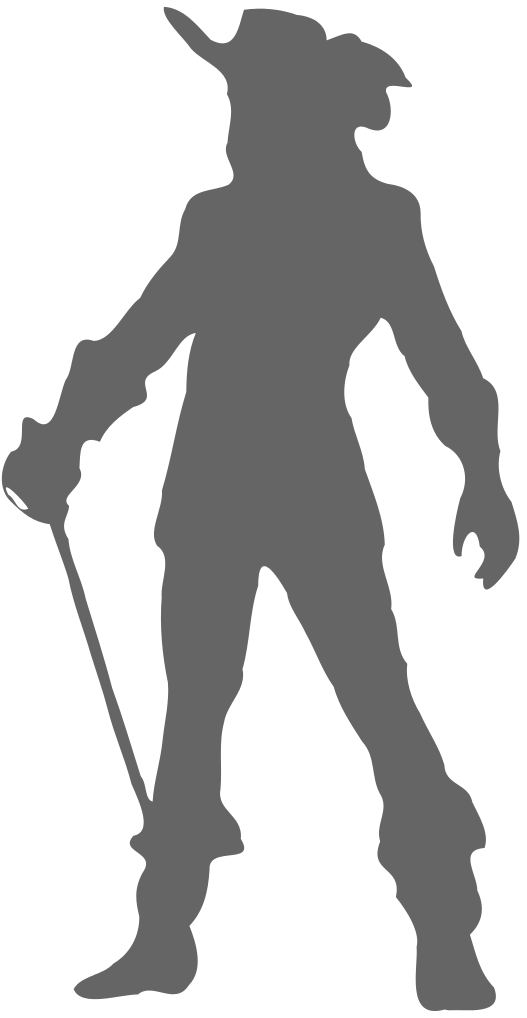
\includegraphics[width=6cm]{../img/silhouette.png}};
        \end{scope}

        \node(kopf) at (3.4, 10) {\RS{\KamRusZonKopf}};
        \begin{scope}[on background layer]
            \path[fill=white, draw=black] ([yshift=0.1cm, xshift=0.2cm]kopf.north west) -- ([xshift=0.2cm]kopf.west) to[out=270, in=155] ([yshift=-0.1cm]kopf.south) to[out=25, in=270] ([xshift=-0.2cm]kopf.east) -- ([yshift=0.1cm, xshift=-0.2cm]kopf.north east) -- cycle;
        \end{scope}
        \node[below=2pt of kopf] {Ko};

        \filldraw[fill=white, draw=black] ([yshift=0.4cm]kopf.north) circle (0.2cm);
        \filldraw[fill=white, draw=black] ([yshift=0.4cm, xshift=0.5cm]kopf.north) circle (0.2cm);
        \filldraw[fill=white, draw=black] ([yshift=0.4cm, xshift=-0.5cm]kopf.north) circle (0.2cm);

        \node(brust) at (2.7, 8) {\RS{\KamRusZonBrust}};
        \begin{scope}[on background layer]
            \path[fill=white, draw=black] ([yshift=0.1cm, xshift=0.2cm]brust.north west) -- ([xshift=0.2cm]brust.west) to[out=270, in=155] ([yshift=-0.1cm]brust.south) to[out=25, in=270] ([xshift=-0.2cm]brust.east) -- ([yshift=0.1cm, xshift=-0.2cm]brust.north east) -- cycle;
        \end{scope}
        \node[below=2pt of brust] {Br};
        \node[right=-4pt of brust](rucken) {\RS{\KamRusZonRucken}};
        \begin{scope}[on background layer]
            \path[fill=white, draw=black] ([yshift=0.1cm, xshift=0.2cm]rucken.north west) -- ([xshift=0.2cm]rucken.west) to[out=270, in=155] ([yshift=-0.1cm]rucken.south) to[out=25, in=270] ([xshift=-0.2cm]rucken.east) -- ([yshift=0.1cm, xshift=-0.2cm]rucken.north east) -- cycle;
        \end{scope}
        \node[below=2pt of rucken] {Rü};

        \filldraw[fill=white, draw=black] ([yshift=0.4cm]$(brust.north)!0.5!(rucken.north)$) circle (0.2cm);
        \filldraw[fill=white, draw=black] ([yshift=0.4cm, xshift=0.5cm]$(brust.north)!0.5!(rucken.north)$) circle (0.2cm);
        \filldraw[fill=white, draw=black] ([yshift=0.4cm, xshift=-0.5cm]$(brust.north)!0.5!(rucken.north)$) circle (0.2cm);

        \node(larm) at (5.6, 6.4) {\RS{\KamRusZonLinkerArm}};
        \begin{scope}[on background layer]
            \path[fill=white, draw=black] ([yshift=0.1cm, xshift=0.2cm]larm.north west) -- ([xshift=0.2cm]larm.west) to[out=270, in=155] ([yshift=-0.1cm]larm.south) to[out=25, in=270] ([xshift=-0.2cm]larm.east) -- ([yshift=0.1cm, xshift=-0.2cm]larm.north east) -- cycle;
        \end{scope}
        \node[below=2pt of larm] {LA};

        \filldraw[fill=white, draw=black] ([yshift=0.5cm, xshift=0.1cm]larm.north west) circle (0.2cm);
        \filldraw[fill=white, draw=black] ([yshift=1cm, xshift=-0.15cm]larm.north west) circle (0.2cm);
        \filldraw[fill=white, draw=black] ([yshift=1.5cm, xshift=-0.4cm]larm.north west) circle (0.2cm);

        \node(rarm) at (0.5, 6.7) {\RS{\KamRusZonRechterArm}};
        \begin{scope}[on background layer]
            \path[fill=white, draw=black] ([yshift=0.1cm, xshift=0.2cm]rarm.north west) -- ([xshift=0.2cm]rarm.west) to[out=270, in=155] ([yshift=-0.1cm]rarm.south) to[out=25, in=270] ([xshift=-0.2cm]rarm.east) -- ([yshift=0.1cm, xshift=-0.2cm]rarm.north east) -- cycle;
        \end{scope}
        \node[below=2pt of rarm] {RA};

        \filldraw[fill=white, draw=black] ([yshift=0.2cm, xshift=0.1cm]rarm.north east) circle (0.2cm);
        \filldraw[fill=white, draw=black] ([yshift=0.6cm, xshift=0.5cm]rarm.north east) circle (0.2cm);
        \filldraw[fill=white, draw=black] ([yshift=1cm, xshift=0.9cm]rarm.north east) circle (0.2cm);

        \node(bauch) at (3, 6) {\RS{\KamRusZonRechterArm}};
        \begin{scope}[on background layer]
            \path[fill=white, draw=black] ([yshift=0.1cm, xshift=0.2cm]bauch.north west) -- ([xshift=0.2cm]bauch.west) to[out=270, in=155] ([yshift=-0.1cm]bauch.south) to[out=25, in=270] ([xshift=-0.2cm]bauch.east) -- ([yshift=0.1cm, xshift=-0.2cm]bauch.north east) -- cycle;
        \end{scope}
        \node[below=2pt of bauch] {Ba};

        \filldraw[fill=white, draw=black] ([yshift=0.4cm]bauch.north) circle (0.2cm);
        \filldraw[fill=white, draw=black] ([yshift=0.4cm, xshift=0.5cm]bauch.north) circle (0.2cm);
        \filldraw[fill=white, draw=black] ([yshift=0.4cm, xshift=-0.5cm]bauch.north) circle (0.2cm);

        \node(rbein) at (1.9, 1.5) {\RS{\KamRusZonRechterArm}};
        \begin{scope}[on background layer]
            \path[fill=white, draw=black] ([yshift=0.1cm, xshift=0.2cm]rbein.north west) -- ([xshift=0.2cm]rbein.west) to[out=270, in=155] ([yshift=-0.1cm]rbein.south) to[out=25, in=270] ([xshift=-0.2cm]rbein.east) -- ([yshift=0.1cm, xshift=-0.2cm]rbein.north east) -- cycle;
        \end{scope}
        \node[below=2pt of rbein] {RB};

        \filldraw[fill=white, draw=black] ([yshift=0.8cm, xshift=0.2cm]rbein.north) circle (0.2cm);
        \filldraw[fill=white, draw=black] ([yshift=1.6cm, xshift=0.3cm]rbein.north) circle (0.2cm);
        \filldraw[fill=white, draw=black] ([yshift=2.4cm, xshift=0.4cm]rbein.north) circle (0.2cm);

        \node(lbein) at (5.1, 1.3) {\RS{\KamRusZonRechterArm}};
        \begin{scope}[on background layer]
            \path[fill=white, draw=black] ([yshift=0.1cm, xshift=0.2cm]lbein.north west) -- ([xshift=0.2cm]lbein.west) to[out=270, in=155] ([yshift=-0.1cm]lbein.south) to[out=25, in=270] ([xshift=-0.2cm]lbein.east) -- ([yshift=0.1cm, xshift=-0.2cm]lbein.north east) -- cycle;
        \end{scope}
        \node[below=2pt of lbein] {LB};

        \filldraw[fill=white, draw=black] ([yshift=0.8cm, xshift=-0.3cm]lbein.north) circle (0.2cm);
        \filldraw[fill=white, draw=black] ([yshift=1.6cm, xshift=-0.6cm]lbein.north) circle (0.2cm);
        \filldraw[fill=white, draw=black] ([yshift=2.4cm, xshift=-0.9cm]lbein.north) circle (0.2cm);
    \end{tikzpicture}
}

\input{kampfbogen-konfig.tex}

\end{dsaCharacterSheet}